%! Author = Luis
%! Date = 26.01.2024


\chapter{Planung und Entwurf}\label{ch:planung-und-entwurf}


\section{Organisation}\label{sec:organisation}
Da ich nicht im Team arbeite, ist die Organisation trivial.
Um einen groben und flexiblen Plan zu haben, orientierte ich mich an Scrum und verwendete einen Backlog mit User-Stories.
Eine Unterteilung in Product Backlog und Sprint Backlog war hier nicht angebracht.
Die Eintr{"a}ge (User Stories) im Backlog sind nicht technisch, sondern fachlich.
Sie folgen einem einheitlichen Schema:
\begin{center}
    Als ``Rolle'' m{"o}chte ich ``Ziel/Wunsch'' (, um ``Nutzen'').
\end{center}

\subsection{User Rollen}\label{subsec:user-rollen}
Ich verwende drei einfache Rollen, um Personen zu klassifizieren, die mit der Anwendung interagieren:
\begin{itemize}
    \item Visitor - jemand der die Seite nur besucht.
    \item User - jemand der einen Account hat.
    \item Admin - jemand der die Seite verwaltet.
\end{itemize}

\subsection{User Stories}\label{subsec:user-stories}

\begin{CheckList}{Task}
    \Task{done}{Als Visitor m{"o}chte ich meine IP-Adresse teilen, um sie auf einem andern Ger{"a}t abzurufen.}
    \Task{done}{Als Visitor m{"o}chte ich {"u}ber die Risiken des Teilens, informiert werden.}
    \Task{open}{Als Visitor m{"o}chte ich {"u}ber das Anlegen eines Users informiert werden.} %todo Texte auf Register Seite Fehlen.
    \Task{done}{Als Visitor m{"o}chte ich einen Accout registirern, um User zu werden.}
    \Task{done}{Als Visitor m{"o}chte ich die App ohne Cookies nutzen k{"o}nnen.}
    \Task{done}{Als Admin m{"o}chte ich eine requirements.txt.}
    \Task{done}{Als User m{"o}chte ich eine Liste aller meiner IPs sehen.}
    \Task{done}{Als User m{"o}chte ich meine IP Passwort gesch{"u}tzt teilen.}
    \Task{started}{Als User m{"o}chte ich sehen wann die IP geteilt wurde.}
    \Task{open}{Als User m{"o}chte ich leicht herausbekommen wie ich die API verwenden kann.} % (Immer hinweise wie ich die Informationen mit der API abrufen k{"o}nnte?!)
    \Task{done}{Als User m{"o}chte ich mich anmelden.}
    \Task{done}{Als User m{"o}chte ich meinen account l{"o}schen k{"o}nnen.}
    \Task{done}{Als User m{"o}chte ich meinen Passwort {"a}ndern k{"o}nnen.}
    \Task{done}{Als User m{"o}chte ich meinen Remember Cookie einstellen k{"o}nnen.}
    \Task{done}{Als User m{"o}chte ich meine Token invalidieren k{"o}nnen.}
    \Task{dropped}{Als User m{"o}chte ich meine Adressen ver{"o}ffentlichen k{"o}nnen.} % -> kein ver{"o}ffentlichen beliebiger Inhalte.
    \Task{done}{Als User m{"o}chte ich {"o}ffentliche IPs importieren/benennen.}
    \Task{done}{Als User m{"o}chte ich Adressen manuell eingeben k{"o}nnen.}
    \Task{open}{Als User m{"o}chte ich IPv4, IPv6 und Url validiert bekommen.}
    \Task{open}{Als User m{"o}chte ich meine Adressen in Gruppen teilen k{"o}nnen.}
    \Task{done}{Als User m{"o}chte ich meine Adressen als QR-Code angezeigt bekommen.}
    \Task{open}{Als Admin m{"o}chte ich eine Firewall.}
    \Task{open}{Als Admin m{"o}chte ich AGB und Datenschutzerkl{"a}rung nutzen.}
    \Task{open}{Als Admin m{"o}chte ich IPs GEO blocken bzw. differenzieren.}
    \Task{done}{Als User m{"o}chte ich meine Aderssen automatisch aktualisiert haben.}
    \Task{done}{Als Admin m{"o}chte ich Rate Limits auf den Routen, um vor DOS-Attacken gesch{"u}tzt zu werden.}
    \Task{dropped}{Als User m{"o}chte ich einen Cookie banner.}
    \Task{started}{Als Visitor m{"o}chte ich keine Cookies.}
    \Task{open}{Als User m{"o}chte ich {"u}ber E-Mail informiert werden k{"o}nnen, wenn der Service nicht verf{"u}gbar ist oder sich {"a}ndert.}
    \Task{unclear}{Als User m{"o}chte ich einen Reverse VPN {"o}ffnen k{"o}nnen.}
    \Task{done}{Als User m{"o}chte ich mein Adressen einfach mit API abrufen k{"o}nnen.}
    \Task{open}{Als User und Visitor m{"o}chte ich ein {"u}bersichtliches Interface.}
    \begin{CheckList}{Task}
        \Task{done}{Als User und Visitor m{"o}chte ich die Public von der Private Tabele unterscheiden können.}
        \Task{open}{Als User und Visitor m{"o}chte ich Mehrsprachigkeint. (Englisch und Deutsch evtl. weitere)}
        \Task{done}{Als User und Visitor m{"o}chte ich durch klicken Adressen und Namen Kopieren.}
        \Task{open}{Als User und Visitor m{"o}chte ich das Teilen durch klicken auf IP klar vermittelt bekommen.}
        \Task{open}{Als User und Visitor m{"o}chte ich Tooltips.}
    \end{CheckList}
    \Task{unclear}{Als Visitor m{"o}chte ich das es schwer oder unm{"o}glich ist, einen Link zu erstellen der automatisch/unfreiwillig meine Adresse teilt.}
    \Task{unclear}{Als Admin m{"o}chte ich Datenbank-Migrationen.}
    \Task{done}{Als Admin m{"o}chte ich Blueprints.}
    \Task{open}{Als Admin m{"o}chte ich Logging, um Angriffe und Fehler zu erkennen.}
    \Task{open}{Als User m{"o}chte ich eine Weiterleitung zur Adresse {"u}ber den Device Namen.}
\end{CheckList}


\section{Frameworks und Entwicklungsumgebung}\label{sec:frameworks-und-entwicklungsumgebung}
Ich verwende Flask als Framework und programmiere in PyCharm Professional 2023.
Ich verwalte mein Python Environment und meine Pakete mit Anaconda\cite{anaconda}.
Die verwendete Python Version ist 3.11.5.
Zur Versionierung verwende ich git und GitHub.
Die verwendeten Bibliotheken und deren Versionen finden sich im environment.yml oder im requirements.txt.
Hier eine kurze {"U}bersicht:

\begin{samepage}
    \begin{itemize}
        \setlength\itemsep{-0.4em}
        \item Flask
        \begin{itemize}
            \setlength\itemsep{-0.4em}
            \item APScheduler
            \item Bcrypt
            \item Limiter
            \item Login
            \item SocketIO
            \item SQLAlchemy
            \item WTF
        \end{itemize}
        \item NumPy
        \item OpenCV
        \item qrcode
        \item Pillow
        \item Requests
        \item PyJWT
        \item urllib3
        \item pytest
    \end{itemize}
\end{samepage}

\section{Datenbankstruktur}\label{sec:datenbankstruktur}
Die Datenbank ist relativ simple.
Es gibt eine User- und eine Address-Tabelle.
Es gelten unter anderem folgende Abh{"a}ngigkeiten:

\begin{align}
    id ~ &\dot \rightarrow ~ passwort \\
    id ~ &\dot \rightarrow ~ remember \\
    id ~ &\dot \leftrightarrow ~ alternative\_id \\
    id ~ &\dot \leftrightarrow ~ name \\
    id, device\_name ~ &\dot \rightarrow ~ address \\
    id, device\_name ~ &\dot \rightarrow ~ last\_updated
\end{align}

\begin{minipage}{0.425\textwidth}
    Abbildung~\ref{fig: db} zeigt das Entity-Relationship-Modell der Datenbank.
    Zwischen shared\_addresses und user besteht eine nur-eins-zu-null-oder-mehr-Beziehung.
    Der Fremdschl{"u}ssel user ist gleich der id in der user-Tabelle.
    Der name ist eindeutig und daher auch Schl{"u}sselkandidat der Tabelle.
    Auch die alternative\_id ist ein eindeutiger Schl{"u}sselkandidat.
    Alle drei id, alternative\_id und name determinieren sich gegenseitig.
\end{minipage}
\hspace{0.05\textwidth}
\begin{minipage}{0.425\textwidth}
    \centering
    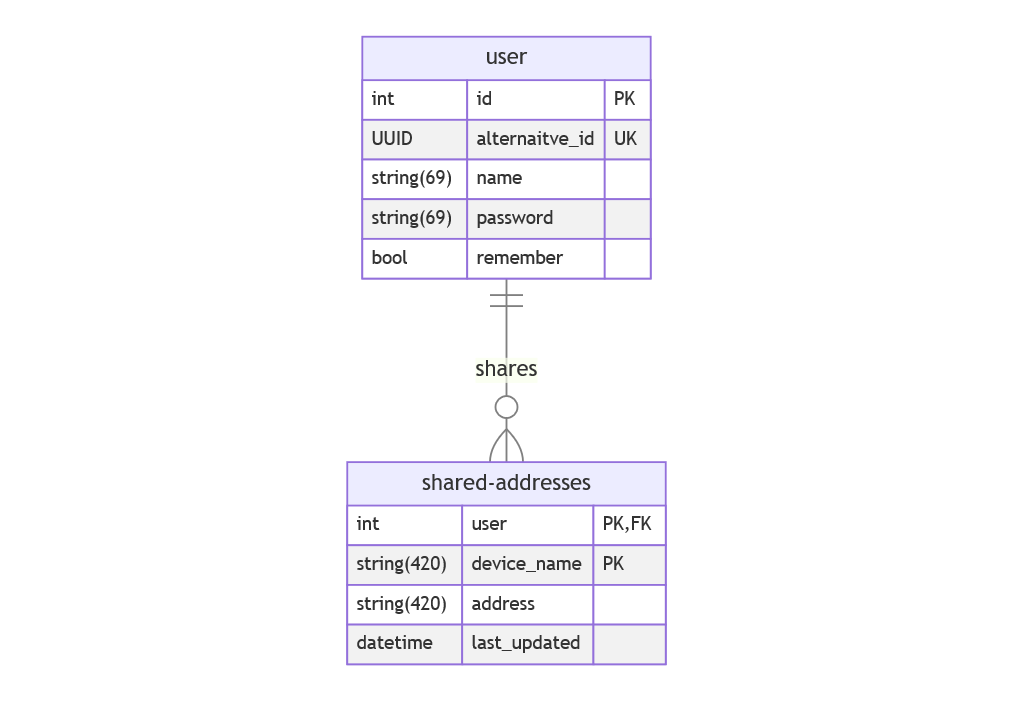
\includegraphics[width=0.6\textwidth]{db}
    \captionof{figure}{Entity-Relationship-Modell der DB}
    \label{fig: db}
\end{minipage}

\vspace{2cm}



Wie Tabelle~\ref{tab: nf-addr} und Tabelle~\ref{tab: nf-user} zeigen sind beide Relationen in 4ter Normalform.
Eine {"U}berf{"u}hrung in die 5te Normalform ist hier nicht n{"o}tig da die Relationen keine mehrwertigen Abh{"a}ngigkeiten haben.
Dementsprechend lassen sich durch eine Teilung auch keine neuen Informationen gewinnen.

\begin{table}[h]
    \centering
    \begin{tabular}{c|c|l}
        \textbf{Normalform} & \textbf{ok/nok} & \textbf{Begr{"u}ndung} \\
        \hline
        1NF & ok & \parbox{10cm}{Alle Dom{"a}nen enthalten nur einfache atomare Werte.} \\
        \hline
        2NF & ok & \parbox{10cm}{address und last\_updated sind voll funktional abh{"a}ngig von (id, device\_name).} \\
        \hline
        3NF & ok & \parbox{10cm}{Es gibt keine transitive Abh{"a}ngigkeit.} \\
        \hline
        BCNF & ok & \parbox{10cm}{Die Determinante (id, device\_name) ist auch Schl{"u}sselkandidat.} \\
        \hline
        4NF & ok & \parbox{10cm}{Es gib keine mehrwertige Abh{"a}ngigkeit.} \\
        \hline
        5NF & nok & \parbox{10cm}{Eine Teilung in address(id, device\_namem, address) und updated(id, device\_namem, last\_updated) w{"a}re m{"o}glich.} \\
    \end{tabular}
    \caption{Normalformen shared\_addresses}
    \label{tab: nf-addr}
\end{table}


\begin{table}[h]
    \centering
    \begin{tabular}{c|c|l}
        \textbf{Normalform} & \textbf{ok/nok} & \textbf{Begr{"u}ndung} \\
        \hline
        1NF & ok & \parbox{10cm}{Passwort k{"o}nnte vom Salt getrennt werden.} \\
        \hline
        2NF & ok & \parbox{10cm}{password und remember sind voll funktional abh{"a}ngig von z.B. id.} \\
        \hline
        3NF & ok & \parbox{10cm}{Es gibt transitive Abh{"a}ngigkeiten nur {"u}ber die Schl{"u}sselkandidaten.} \\
        \hline
        BCNF & ok & \parbox{10cm}{Jede der drei Determinanten ist auch Schl{"u}sselkandidat.} \\
        \hline
        4NF & ok & \parbox{10cm}{Es gib keine mehrwertige Abh{"a}ngigkeit.} \\
        \hline
        5NF & nok & \parbox{10cm}{Teilung in Alternative(id, alternative\_id), Name(id, name), Password(id, password) und Remember(id, remember) m{"o}glich.} \\
    \end{tabular}
    \caption{ Normalformen user}
    \label{tab: nf-user}
\end{table}
